\documentclass[12pt]{memoireuqam1.3}

\usepackage{graphicx}% Pour les figures
\usepackage[french]{babel}
\usepackage[utf8]{inputenc} % Pour utiliser les caractères accentués
\usepackage[T1]{fontenc}
\usepackage{hyperref}
\usepackage{listings}
\usepackage{float}
\usepackage{caption}
\usepackage{chngcntr}
\usepackage{lscape}

\usepackage{color}

\definecolor{Gray}{RGB}{245,245,245}
\definecolor{CPPGray}{RGB}{120,120,120}

\lstdefinestyle{default}{
  showspaces=false,
  showtabs=false,
  breaklines=true,
  showstringspaces=false,
  breakatwhitespace=true,
  basicstyle=\ttfamily,
  backgroundcolor=\color{Gray},
  numbers=left, numbersep=3pt, stepnumber=1, numberstyle=\tiny\color{CPPGray},
  rulecolor=\color{CPPGray},
  basicstyle=\footnotesize
}

\definecolor{dkblue}{rgb}{0,0,.6}

\lstset{language=php,
  keywordstyle = \color{dkblue},
  style=default}

\newfloat{lstfloat}{h}{lstfloat} %Instancie la liste des exemples de codes
\floatname{lstfloat}{Code} %Associe le nom Code à la liste des exemples de codes
\counterwithin{lstfloat}{chapter} %Numérote bien les exemples de codes

\newcommand\listcodename{Liste des exemples de code}
\newcommand\listofcodes{% Pris de memoireuqam1.3.cls
{
    \listof{lstfloat}{\listcodename}
    \addtocontents{toc}{\protect\vspace{1.5ex}}
    \addcontentsline{toc}{chapter}{\UpperRef{\listcodename}}
    }
}

%\input macro  % Pour les définitions personnelles

\newcommand{\GT}[1]{{\footnotesize\textcolor{red}{[[(GT) #1]]}}}

\definecolor{darkgreen}{rgb}{0.0, 0.35, 0.0}
\newcommand{\PG}[1]{{\footnotesize\textcolor{darkgreen}{[[(PG) #1]]}}}


\begin{document}

%%%%%%%%%%%%%%%%%%%%
% Pour la page titre
%%%%%%%%%%%%%%%%%%%%
\title{Développement d'un module d'extension Moodle d'aide à la correction de questions de type \og texte~long \fg{}}
% Votre nom complet tel qu'il apparaît à votre dossier du registrariat de l'UQAM
\author{Philippe Girard}
% Année et mois courant sauf si spécifié autrement pas \degreemonth et \degreeyear
%\degreemonth{mois du dépôt}
%\degreeyear{année du dépôt}
\uqamprojet %\uqammemoire %% ou \uqamthese ou \uqamrapport
\matiere{Génie logiciel}


\thispagestyle{empty}        % La page titre n'est pas numérotée
\maketitle

%%%%%%%%%%%%%%%%%%%%
% Page préliminaires
%%%%%%%%%%%%%%%%%%%%
% \renewcommand \bibname{R\'EF\'ERENCES}% FACULTATIF
%si vous voulez qu'apparaisse le titre RÉFÉRENCES plutôt que BIBLIOGRAPHIE

\renewcommand \listfigurename{LISTE DES FIGURES}
\renewcommand \appendixname{APPENDICE}
\renewcommand \figurename{Figure}
%\renewcommand \tablename{Tableau}

\pagenumbering{roman} % numérotation des pages en chiffres romains
\addtocounter{page}{1} % Pour que les remerciements commencent à la page ii
\chapter*{Remerciements}

Premi\`erement, j'aimerais remercier mon directeur de ma\^itrise, M. Guy Tremblay.
Sans son support, ce projet n'aurait pas \'et\'e un succ\`es.
Je tiens aussi \`a souligner sa disponibilit\'e pour la tenue de nos rencontres \`a l'ext\'erieur de l'UQAM.

Merci aussi au C\'egep R\'egional de Lanaudi\`ere, \`a Joliette, qui m'a aid\'e au niveau financier dans ce projet.

J'aimerais aussi remercier mes parents et amis, qui ont su croire en ce projet malgr\'e une date de fin toujours repouss\'ee.
Mention sp\'eciale \`a Marc-Andr\'e, qui m'a aid\'e \`a rester motiv\'e tout au long du projet.

\tableofcontents % Pour générer la table des matières
\listoftables % Pour générer la liste des tableaux
\listoffigures % Pour générer la liste des figures
\listofcodes % Pour générer la liste des exemples de code
\begin{abstract}

Ce projet consiste à développer un module d'extension (\textit{plugin}) Moodle pour aider la correction des textes à développement dans une activité de type \og questionnaire \fg{}.

Le module d'extension développé est de type \og Type de question \fg{} basé sur le module d'extension \og \textit{qtype\_essay} \fg{}.
Le nouveau type de question se comporte  comme le type \og \textit{qtype\_essay} \fg{} hormis qu'il ne permet pas la remise de fichiers ou l'utilisation du \textit{WYSIWYG (What You See Is What You Get)}.
Plus sp\'ecifiquement, ce nouveau module ajoute les fonctionnalités suivantes au module de correction manuelle: mise en évidence de mots-clés trouvés par racination (\textit{stemming}) et affichage de la réponse de l'enseignant adjacent à la réponse de l'étudiant.

Des tests unitaires ainsi que des tests d'acceptation ont été écrits afin de valider le fonctionnement de ce module d'extension.

Les fonctionnalités de ce module d'extension sont limit\'ees. 
Notamment, des ajouts tels que les suivants seraient utiles pour apporter une aide plus importante au correcteur: remplacer la racination pour la lemmatisation afin d'améliorer l'identification des mots-clés~; comparer les textes des étudiants entre eux afin de détecter le plagiat~; effectuer une analyse syntaxique afin de donner une estimation de la note que mérite un texte basé sur les réponses précédemment corrigées.

MOTS-CLÉS: Moodle, Tests unitaires, Tests d'acceptation, Racination

\end{abstract}

% Utilisez l'environnement  abstract pour rédiger votre résumé


%%%%%%%%%%%%%%%%%%%%
% Document principal
%%%%%%%%%%%%%%%%%%%%

\begin{introduction}

L'id\'ee pour ce projet est n\'ee d'une discussion entre mon directeur de recherche, M.\ Guy Tremblay, et la professeure Magda Fusaro.
Mme Fusaro enseignait alors un cours o\`u les \'etudiants et les \'etudiantes devraient rendre plusieurs petits travaux de r\'edaction sur Moodle.
La correction de ces nombreux travaux \'etait un travail fastidieux qui prenait de nombreuses heures.

Plus pr\'ecis\'ement, les \'etudiants et les \'etudiantes devaient \'ecrire un document Word et l'envoyer sur Moodle.
Or, la correction d'un texte dans un document Word, o\`u tout est possible au niveau contenu et de la mise en forme, est complexe,  et les \'etudiants et les \'etudiantes peuvent facilement ne pas respecter le gabarit m\^eme lorsqu'il leur est fourni.
Nous avons donc convenu de r\'ealiser notre projet imm\'ediatement dans Moodle au lieu de faire un outil externe, car Moodle permet de faire un questionnaire en ligne qui est facilement balisable.

Moodle est une plateforme utilisée par plusieurs établissements scolaires au Québec, notamment, la plupart des cégeps et quelques universités l'offrent à leurs enseignants.
J'ai d'ailleurs eu à utiliser cette plateforme en tant qu'étudiant à l'Université du Québec à Montréal et aussi en tant qu'enseignant au Cégep Régional de Lanaudière à Joliette.

Moodle permet, entre autres, de créer et de corriger des travaux, quiz ou examens en ligne.
La correction est une tâche complexe et g\'en\'eralement peu appréciée par les enseignants et enseignantes.
L'idée générale de ce projet est donc d'aider les enseignants et correcteurs dans leur tâche de correction à l'intérieur d'un environnement Moodle.
Plus sp\'ecifiquement, le but du projet \'etait de créer un module d'extension Moodle d'aide à la correction des textes à développement qui permet, entre autres, la mise en évidence de mots-clés sp\'ecifi\'es par l'enseignant.

Ce document pr\'esente les principales étapes de réalisation du projet.
Premièrement, nous avons d\^u en apprendre plus sur Moodle en tant que correcteur et en tant que programmeur afin de créer le bon type de module d'extension.
Deuxièmement, nous avons d\^u trouver les méthodes de détection de mots-clés et choisir celle qui semblait la plus appropri\'ee.
Troisièmement, nous avons d\^u comprendre comment tester notre module d'extension selon les bonnes pratiques de la plateforme Moodle.
Finalement, nous avons développ\'e et test\'e notre module d'extension.

\end{introduction}

% Utilisez l'environnement  introduction pour rédiger votre introduction
\chapter{Introduction à Moodle}

Moodle est un environnement d'apprentissage en ligne (LMS, Learning Management System) développé par Martin Dougiamas. Cette plateforme est un logiciel libre développé en PHP sous \href{http://docs.moodle.org/dev/License}{licence GPL (GNU Public License)} dont le code source se trouve sur \href{https://github.com/moodle/moodle}{GitHub}.

Moodle est un outil très modulaire, chaque enseignant peut créer ses cours comme il le souhaite. Chaque cours est séparé en sections définies en semaine, module, thème ou plusieurs autres configurations possibles. Pour chaque section on peut créer des activités: un texte à lire, des documents à télécharger, un forum, un sondage, un questionnaire en ligne, un devoir à remettre et plus encore. Chaque activité est hautement configurable. Par exemple, un devoir peut être fait individuellement ou en équipe, avoir une date et une heure de début et de fin de disponibilité avec un délai de retard permis. Dans les questionnaires en ligne un enseignant peut créer une banque de questions et sélectionner les questions désirées ou laisser le système en choisir aléatoirement.

\section{Activité questionnaire}

Ce projet s'attarde à l'activité Questionnaire de Moodle, plus spécifiquement sur la question de type Texte long (parfois appelé Composition, selon la version de Moodle). Tout d'abord, qu'est-ce qu'une activité Questionnaire? Cette activité permet à l'enseignant de créer un formulaire en ligne auquel les étudiants devront répondre. Il peut s'agir, par exemple, d'une évaluation sommative qui sera cumulée au carnet de notes Moodle, d'une évaluation formative ou d'un atelier qui pourra être refait plusieurs fois jusqu'à ce que l'étudiant atteigne une note prédéfinie.

Parmi les options les plus utiles de cette activité nous avons (toutes optionnelles): Début et fin de disponibilité du questionnaire, le temps disponible à partir de l'ouverture du questionnaire, note pour passer, mélanger aléatoirement les questions, nombre de tentatives possibles, etc.

Chaque questionnaire est composé d'un nombre de questions choisies dans une banque de questions. Les questions peuvent avoir un ordre précis ou être choisies aléatoirement parmi un ensemble de questions. Voici une liste non exhaustive des types de questions:

\begin{description}
  \item[Choix multiple]
  
  Génère une liste de boutons radio ou de case à cocher. Chaque bouton vaut un nombre de points entre -100\% et 100\% de la valeur de la question.
  
  \item[Réponse courte]
  
  Affiche un champ texte corrigé à l'aide de réponses possibles ou d'expression régulière
  
  \item[Numérique]
  
  Affiche un champ texte pour valeur numérique pouvant prendre en compte une unité de mesure (km, cm et m par exemple).
  
  \item[Question Cloze]
  
  Permets de créer un texte troué permettant plusieurs sous-questions de types choix multiples, réponse courte et numérique.
  
  \item[Composition]
  
  Affiche un champ texte multiligne, multiligne avec police monospace ou WYSIWYG (What You See Is What You Get). L'étudiant doit écrire un texte à développement.
\end{description}

\section{Question de type Composition}

Dû à sa nature, le type de question Composition est le seul qui ne peut pas se corriger automatiquement par Moodle. L'enseignant doit donc corriger manuellement toutes les réponses. Heureusement, Moodle inclut un module de correction manuelle qui permet au correcteur de corriger les questions de ce type. L'enseignant peut choisir de corriger étudiant par étudiant, évaluant chaque question d'un étudiant une après l'autre. Il peut aussi corriger question par question, la réponse de tous les étudiants à une question se retrouve sur une seule page, une en dessous de l'autre. Cette dernière méthode est très appréciée de certains enseignants, car elle permet de comparer toutes les réponses données et ainsi corriger de manière juste.

Ce projet consiste donc de faciliter le travail du correcteur en créant un nouveau module Moodle qui:

\begin{enumerate}
  \item Affichera la réponse de l'étudiant et la réponse de l'enseignant côte à côte afin de faciliter la tâche au correcteur.
  \item Surlignera les mots clés donnés par l'enseignant dans la réponse de l'étudiant et de l'enseignant
  \item Utilisera la racination ou la lemmisation afin de surligner les mots, peu importe leur accord
\end{enumerate}

L'extension sera donc utile pour les questions à développement pour les textes descriptifs et pour des fonctions de programmations, mais le sera moins pour les textes d'opinion où il n'y a pas de \og bonne \fg{} réponse.
\chapter{D\'etection des mots-cl\'es}
\label{chap:keywords}
\PG{Je n'ai malheureusement aucune r\'ef\'erence qui appuie mon choix de prendre la lemmatization ou le stemming pour la d\'etection de mots cl\'es.
Dois-je continuer mes recherches pour trouver une source ou dans ma conclusion j'indique mon manque de recherche avant de commencer?}
Afin d'identifier les mots-cl\'es pr\'esents dans le texte d'un \'etudiant et les comparer avec ceux fournis par l'enseignant, nous avons d\'ecid\'e d'utiliser la racine de chaque mot.
En utilisant la racine de chaque mot, nous pouvons trouver les mots-cl\'es, peu importe leur accord ou le temps de verbe.
Deux techniques de recherche de racine d'un mot ont \'et\'e retenues: la lemmatisation et la racination (\textit{stemming}).
\GT{Je crois qu'il pourrait \^etre int\'eressant d'illustrer \`a quoi
ressemble un petit programme Snowball. De plus, la distinction entre
Snowball et php-stemmer n'est pas claire: ce dernier s'inspire
simplement de Snowball pour l'algorithme ou utilise directement le
langage?}
Lors du choix de la technique utilis\'ee, nous avons pris en consid\'eration les points suivants:
\begin{enumerate}
  \item Le but du projet n'\'etant pas de faire de l'analyse linguistique, une biblioth\`eque devra \^etre utilis\'ee si possible;
  \item La biblioth\`eque doit \^etre \'ecrite en PHP, langage utilis\'e par Moodle, afin de faciliter l'installation du module d'extension d\'evelopp\'e;
  \item La biblioth\`eque doit permettre de trouver la racine des mots en fran\c{c}ais, en anglais, et en plusieurs autres langues si possible, et ce afin de permettre l'utilisation du module d'extension \`a travers le monde.
\end{enumerate}
\section{La lemmatisation}
La lemmatisation consiste \`a trouver le lemme de chaque mot.
Le lemme est la forme canonique d'un mot, soit l'infinitif pour un verbe, le masculin singulier pour un adjectif, etc.
Par exemple, le lemme du verbe \og aimerait \fg{} est \og aimer \fg{}.
La  technique de lemmatisation utilise habituellement un dictionnaire qui associe toutes les conjugaisons possibles d'un mot \`a leur lemme.
Certaines biblioth\`eques vont m\^eme consid\'erer le contexte afin de trouver le bon lemme.
Les biblioth\`eques de lemmatisation \'ecrites en PHP sont rares.
Lors de nos recherches, aucune de ces biblioth\`eques ne supportait le fran\c{c}ais et l'anglais.
\section{La racination}
La racination consiste \`a trouver la racine (parfois appel\'e radical, ou \emph{stem} en anglais) de chaque mot.
La racine est trouv\'ee par un algorithme en enlevant la fin du mot.
Par exemple, la racine de \og aimerait \fg{} est \og aim \fg{}.
Cette technique ignore la plupart des exceptions.
La racination est moins pr\'ecise que la lemmatisation.
Par exemple, la racine de \og courons \fg{} est la m\^eme que la racine de \og couronnement \fg{}, soit \og couron \fg{}.
La lemmatisation ne fera pas la m\^eme erreur et trouvera les lemmes \og courir \fg{} et \og couronne \fg{}.
En contrepartie, la recherche de la racine sera plus rapide avec un algorithme de racination qu'une recherche dans un dictionnaire de lemmes.
Il existe quelques biblioth\`eques de racination en PHP.
Une d'elles est \texttt{php-stemmer}\cite{phpstemmer} qui fait la racination en fran\c{c}ais, en anglais, et dans dix autres langues.
Les algorithmes utilis\'es par \texttt{php-stemmer} sont une traduction en PHP des algorithmes \'ecrits en Snowball, un langage d\'evelopp\'e pour la racination.
\GT{Il faudrait indiquer une r\'ef\'erence ci-haut. Celle indiqu\'ee
par href n'est pas visible on dirait dans le PDF.}
\PG{J'ai remplac\'e tous les href par des footnote-url. J'ai aussi essay\'e de clarifi\'e le lien entre php-stemmer et Snowball.}
Comme nous avons trouv\'e une biblioth\`eque de racination qui satisfait tous les crit\`eres et aucune biblioth\`eque de lemmatisation n'en fait autant, ce projet va utiliser \texttt{php-stemmer} pour la d\'ecouverte de mots-cl\'es.
\section{Snowball}
Snowball est un petit langage de traitement de texte pour la racination de texte.
Une application Snowball peut \^etre compil\'ee en C ou en Java.
Le site web de Snowball donne l'algorithme de racination pour plusieurs langues: anglais, fran\c{c}ais, espagnol, allemand, russe, etc.
Le langage ainsi que l'algorithme pour la langue anglaise ont \'et\'e d\'evelopp\'es par Martin Porter \cite{snowball}.
%
\GT{Pr\'ef\'erable si tu pouvais donner une r\'ef\'erence, avec $\backslash$cite\{...\}, pour cet algorithme.}
%
L'origine des algorithmes pour les langues latines, incluant la langue fran\c{c}aise, n'est pas donn\'ee, mais semble venir aussi de Porter et de contributeurs.
Les algorithmes Snowball sont plut\^ot simples comme on peut le voir \`a l'exemple \ref{code:snowball-exemple}.
Cet exemple ex\'ecute une \'etape pr\'eliminaire \`a la racination, soit la gestion des voyelles.
Les lettres en majuscules ne seront plus consid\'er\'ees comme des voyelles pour la racination.
L'algorithme au complet est disponible \`a l'adresse \href{https://raw.githubusercontent.com/snowballstem/snowball/master/algorithms/french/stem_ISO_8859_1.sbl}.
\begin{lstfloat}
\begin{lstlisting}[frame=l]
define v 'aeiouy{a^}{a`}{e"}{e'}{e^}{e`}{i"}{i^}{o^}{u^}{u`}'
define prelude as repeat goto (
    (  v [ ('u' ] v <- 'U') or
           ('i' ] v <- 'I') or
           ('y' ] <- 'Y')
    )
    or
    (  ['y'] v <- 'Y' )
    or
    (  'q' ['u'] <- 'U' )
)
\end{lstlisting}
\caption{Exemple de l'algorithme de racination en fran\c{c}ais en Snowball.}
\label{code:snowball-exemple}
\end{lstfloat}
\GT{Je crois qu'il y a trop de d\'etails dans ce qui suit.  Je crois
qu'il serait pr\'ef\'erable d'avoir tout d'abord un algorithme <<de
haut niveau>>, i.e., une vue d'ensemble sans trop de d\'etails, par
exemple, avec du pseudocode ou, peut-\^etre m\^eme, avec du code
Snowball si c'est compr\'ehensible. Ensuite, les d\'etails pourraient
\^etre donn\'es, mais soit dans une ou des figures, soit en annexe.
Parce que lorsqu'on lit un rapport/m\'emoire, ce qu'on lit devrait
\^etre du texte relativement <<lisible>>, et pas trop de d\'etails ---
trop d'arbres qui emp\^echent de voir la for\^et!}
\PG{J'ai inclus un peu plus haut un lien vers l'algorithme complet Snowball. Pour un programmeur c'est plus simple \`a comprendre l'algorithme en Snowball que de le lire textuellement. J'ai enlev\'e beaucoup de d\'etail dans le texte ci-dessous, est-ce que le diagramme serait suffisant?}
Les algorithmes Snowball sont structur\'es en plusieurs \'etapes.
Ce qui suit explique les grandes lignes de l'algorithme de racination en fran\c{c}ais qui sont illust\'rées \`a la figure \ref{snowball-process}.
Pour plus d'informations, voir \url{http://snowballstem.org/algorithms/french/stemmer.html}.
\begin{figure}[h!]
  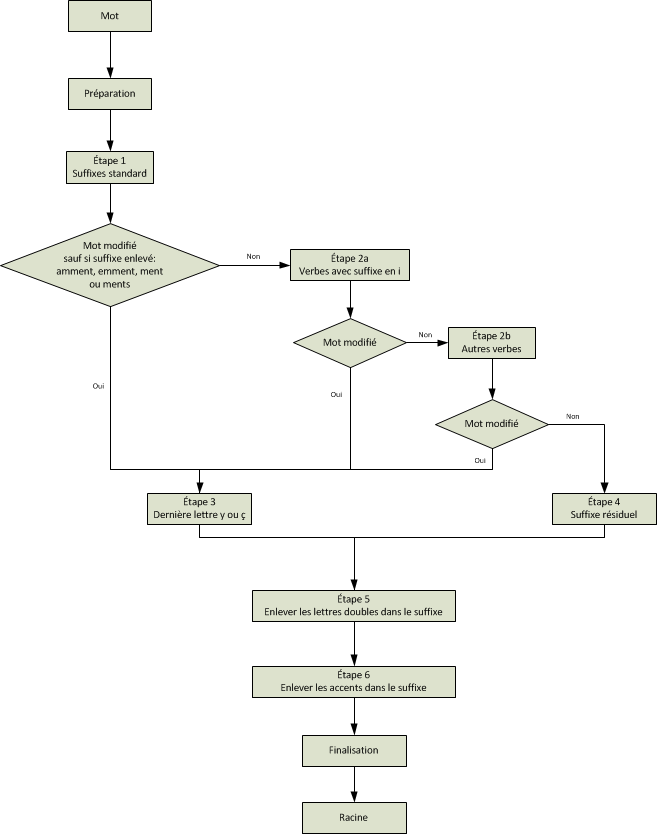
\includegraphics[scale=0.7]{images/snowball.png}
  \caption{Processus de racination Snowball pour la langue fran\c{c}aise.}
  \label{snowball-process}
\end{figure}

\begin{itemize}
\item{Pr\'eparation}
En se basant sur la position des voyelles, on d\'etermine la section du mot qui pourrait \^etre un suffixe.
\item{\'etape 1: Suffixes standards}
Cette \'etape sert \`a trouver la racine des mots, adjectifs, adverbes, etc.
On enl\`eve les suffixes standards (logie, emment, atrice, etc.)
\item{\'etape 2: Suffixes de verbes}
Cette \'etape trouve la racine d'un verbe.
Il faut faire cette \'etape seulement si l'\'etape 1 n'a rien chang\'e ou si un des suffixes suivants a \'et\'e trouv\'e: amment, emment, ment et ments.
\begin{itemize}
\item{\'etape 2a: Suffixes d\'ebutant par i}
On trouve le suffixe qui d\'ebute par i (îmes, ie, ira, etc.)
\item{\'etape 2b: Autres suffixes de verbes}
On trouve le suffixe de verbe (\'e, era, âmes, aient, etc.)
\end{itemize}
\item{\'etape 3: Derni\`ere lettre}
Si les \'etapes 1 ou 2 ont modifi\'e le mot, faire cette \'etape, sinon passer \`a l'\'etape 4.
Si la derni\`ere lettre est un y, la remplacer par i.
Si c'est un \c{c}, la remplacer par c.
\item{\'etape 4: R\'esidue du suffixe}
Il faut faire cette \'etape seulement si les \'etapes 1 \`a 3 n'ont pas modifi\'e le mot.
Cette \'etape sert \`a enlever le pluriel et le f\'eminin des mots proches de leurs racines.
\item{\'etape 5: D\'edoubler la lettre finale}
Les suppressions et remplacements des \'etapes pr\'ec\'edentes peuvent laisser une faute dans la racine du mot.
Cette \'etape sert \`a enlever les lettres doubles de certaines finales de mots (enn, ell, eill, etc.).
\item{\'etape 6: Accent final}
Cette \'etape aussi sert \`a nettoyer la racine du mot.
Si un mot se termine par la lettre \textbf{\`e ou \'e} suivi d'une ou plusieurs consonnes, enlever l'accent de ce \textbf{e}.
\item{Finalisation}
Finalement, on enl\`eve les majuscules sur les voyelles ajout\'ees durant l'\'etape de pr\'eparation.
\end{itemize}
Au final, on obtient la racine du mot.
Lors de la comparaison de texte, il peut y avoir quelques probl\`emes.
Par exemple les mots \og acceptables \fg{} et \og accept\'e \fg{} ont la m\^eme racine: \og accept \fg{}.
Par contre, le sens des deux mots est diff\'erent.

\GT{Tu discutes beaucoup de la racination pour obtenir <<l'essence>>
des mots-cl\'es.  Mais tu n'expliques peut-\^etre pas assez comment
cela est utilis\'e dans ton processus/outil.}
\section{\texttt{php-stemmer} et son utilisation}
Le fichier \textit{README.md} du git de \texttt{php-stemmer} le d\'ecrit : \og \textit{PHP5 native implementation of Snowball stemmer} \fg{} \cite{phpstemmer}.
En comparant le code de la librairie \texttt{php-stemmer} et les algorithmes Snowball nous pouvons remarquer que les algorithmes sont les m\^emes.
\texttt{php-stemmer} est donc une traduction PHP des algorithmes Snowball.
Cette librairie nous servira \`a trouver la racine de chaque mot cl\'e, de chaque mot dans la r\'eponse de l'\'etudiant ainsi que dans chaque mot dans la r\'eponse de l'enseignant.
De cette mani\`ere, il sera possible de mettre en \'evidence chaque mot cl\'e dans la r\'eponse de l'\'etudiant, peu importe l'accord.
Par exemple, si l'enseignant donne \og illumination \fg{} comme mot cl\'e et l'\'etudiant donne la r\'eponse \og Le pont Jacques-Cartier \`a \'et\'e illumin\'e pour le 375\textsuperscript{i\`eme} de la ville de Montr\'eal. \fg{}.
La racine du mot cl\'e \og illumination \fg{}  est \og illumin \fg{}.
En regardant la racine de chaque mot dans la r\'eponse de l'\'etudiant, on remarque que la racine du mot \og illumin\'e \fg{} est aussi \og illumin \fg{}.
Il faudrait donc mettre en \'evidence le mot \og illumin\'e \fg{} lorsqu'on affiche la r\'eponse au correcteur.
Le module d'extension devra afficher la r\'eponse de l'\'etudiant avec le mot ilumi\'e en \'evidence tel qu'illustr\'e dans la phrase suivante: \og Le pont Jacques-Cartier \`a \'et\'e \textbf{\underline{illumin\'e}} pour le 375\textsuperscript{i\`eme} de la ville de Montr\'eal. \fg{} 
\chapter{Tests Moodle}
Moodle offre du support pour deux types de tests: des tests unitaires et des tests d'acceptation.
La plateforme inclut plusieurs centaines de ces deux types de tests automatis\'es d\`es son installation.
Ils seront tous effectu\'es avant le d\'ebut du d\'eveloppement afin de s'assurer que Moodle fonctionne correctement sans le nouveau module d'extension.
Une fois le d\'eveloppement termin\'e, les tests seront effectu\'es de nouveau afin de valider que le nouveau module d'extension ne r\'egresse pas les autres fonctionnalit\'es de Moodle.

L'environnement utilis\'e afin de rouler les tests est une machine virtuelle Xubuntu~16.04 mise \`a jour en date du 14 d\'ecembre~2017.
La version de PHP est la version~7.0.22.
Le moteur de base de donn\'ees est MySQL version~5.7.20 install\'e avec les paquets Ubuntu.
La base de donn\'ees utilise la collation \texttt{utf8mb4\_unicode\_ci} comme conseill\'ee dans la documentation\footnote{\url{https://docs.moodle.org/34/en/MySQL}}.
La version de Moodle est la derni\`ere version stable \`a ce jour, soit la version~3.4.
Moodle a \'et\'e install\'e avec \texttt{git} \`a partir de la branche \texttt{MOODLE\_34\_STABLE}, \textit{commit} a45c466\footnote{\url{https://github.com/moodle/moodle/commit/a45c46600021667691dbb4bce5420a2f65d3239c}} d\'eploy\'e le 14 d\'ecembre~2017.
Les tests ont \'et\'e ex\'ecut\'es une seule fois \textbf{avant} le d\'eveloppement du module d'extension afin de confirmer le fonctionnement de l'environnement.

\section{Tests unitaires}
\label{test-unitaires}
Les tests unitaires effectuent des v\'erifications \`a petite \'echelle.
Chaque fonction dans le code est test\'ee de fa\c{c}on isol\'ee.
Dans certains cas, pour tester de fa\c{c}on isol\'ee une fonction, il faut remplacer les d\'ependances par des \textit{stubs}.
Un \textit{stub} va simuler la d\'ependance utilis\'ee par la fonction en retournant une valeur fixe.
De cette mani\`ere, il est possible de tester cette fonction uniquement sans \^etre impact\'e par les autres fonctions.
Plusieurs tests peuvent \^etre effectu\'es afin de valider tous les cas possibles. \cite{tremblay16}

\begin{lstfloat}[htbp]
\begin{lstlisting}[frame=l]
class qtype_essay_question_test extends advanced_testcase {
    public function test_get_question_summary() {
        $essay = test_question_maker::make_an_essay_question();
        $essay->questiontext = 'Hello <img src="http://example.com/globe.png" alt="world" />';
        $this->assertEquals('Hello [world]', $essay->get_question_summary());
    }
}
\end{lstlisting}
\caption{Exemple de test unitaire du module d'extension \texttt{qtype\_essay}.}
\label{code:unittest}
\end{lstfloat}

Une installation \og vanille \fg\ de Moodle vient avec plusieurs tests unitaires.
Le code de base ainsi que les modules d'extension de base sont d\'ej\`a test\'es.
Ces tests fonctionnent avec \textit{PHPUnit}, un \textit{framework} de tests unitaires pour PHP.
Un exemple de test unitaire est pr\'esent\'e dans l'extrait de code \ref{code:unittest}.
Cet exemple v\'erifie la validit\'e du r\'esum\'e de la question qui est le texte de la question sans images et sans mise en forme.
Le r\'esum\'e de la question va \^etre utilis\'e dans la banque de question, afin de la retrouver facilement dans une liste.


Avant de d\'eployer le module d'extension, la suite de tests \textit{PHPUnit}, fournie avec Moodle, a \'et\'e ex\'ecut\'ee.
Elle comporte 8750 tests et 90~575 v\'erifications (\textit{assertions}) \`a ex\'ecuter.
8682 tests ont r\'eussi (\textit{success}), 67 tests ont \'et\'e ignor\'es (\textit{skipped}) et un test a \'echou\'e (\textit{failures}).
Les tests ignor\'es sont, par exemple, les tests pour LDAP et les tests pour Redis, deux technologies qui n'ont pas \'et\'e configur\'ees dans notre cas.

Il y avait malheureusement une erreur caus\'ee par l'encodage des caract\`eres dans la base de donn\'ees MySQL.
Le test v\'erifie que la base de donn\'ees fonctionne en UTF8 et consid\`ere la casse (\textit{case-sensitive}) lors de la comparaison de texte.
La version de la base de donn\'ees MySQL utilis\'ee pour les tests est 5.7.
Or, il n'y a pas d'encodage UTF8 sensible \`a la casse pour les versions pr\'ec\'edentes \`a MySQL~5.8.
L'erreur est connue et d\'etaill\'ee sur le site de r\'ef\'erence Moodle\footnote{\url{https://docs.moodle.org/dev/Database_collation_issue}}.
Cette erreur peut poser probl\`eme dans les questions de type num\'erique ainsi que pour les remises de fichiers.
Par exemple, on ne peut pas entrer les unit\'es \og km \fg{} et \og Km \fg{} dans les r\'eponses possibles, car la base de donn\'ees consid\`ere ces unit\'es comme \'etant identiques.
Par contre, la correction de la question, ex\'ecut\'ee en PHP, distingue les deux unit\'es.
Un \'etudiant qui r\'epond avec l'unit\'e \og 10~KM \fg{} alors que l'enseignant a enregistr\'e la r\'eponse \og 10~km \fg{} aura donc une erreur.
Comme le module d'extension d\'evelopp\'e n'utilisera pas la comparaison de texte \`a partir de la base de donn\'ees, le d\'eveloppement peut continuer sans probl\`eme.

Si notre application est enti\`erement test\'ee avec des tests unitaires, nous sommes assur\'es qu'il ne devrait pas y avoir de probl\`eme de code dans les fonctions.
Par contre, si on compare les tests \`a une \'equipe sportive, les tests unitaires analysent chaque joueur, mais ne consid\`erent pas le travail d'\'equipe.
Il faut donc ajouter un autre type de test, les tests d'acceptation, afin de s'assurer de l'efficacit\'e du travail d'\'equipe.

\section{Tests d'acceptation}
\label{test_acceptation}
Un test d'acceptation valide que l'application satisfait aux exigences du logiciel.
Ce type de test peut s'ex\'ecuter \`a partir de l'interface, de la m\^eme mani\`ere qu'un humain pourrait tester le logiciel --- il s'agit donc d'un test qui ex\'ecute le logiciel <<de bout en bout>>~\cite{tremblay16}.

Moodle vient aussi avec plusieurs de ces tests, mais ce ne sont pas tous les modules d'extension qui en ont.
%
Les tests d'acceptation sont ex\'ecut\'es \`a l'aide de \texttt{behat}, un \textit{framework} PHP d'automatisation de tests qui se base sur le \og \textit{Behavior Driven Development} (BDD) \fg{}.



Un serveur ou une application Selenium ex\'ecutera les tests en ligne de commande ou dans un navigateur web, selon le besoin.
Les tests sont \'ecrits sous forme textuelle anglaise, g\'en\'eralement compr\'ehensibles par tous les intervenants.
Chaque instruction et v\'erification doit \^etre, pr\'ealablement, configur\'ee en PHP.
La structure des tests d'acceptation avec \texttt{behat} est comme suit (un exemple se trouve à l'annexe~\ref{annexe_behat_exist}, p.~\pageref{annexe_behat_exist}):
\begin{itemize}
  \item La premi\`ere ligne avec les \verb|@| permet de cat\'egoriser chaque fichier de test.
        Ceci permet d'ex\'ecuter les tests d'acceptations pour un seul module d'extension ou pour un type de module d'extension;
        
  \item La ligne d\'ebutant par \textit{Feature} donne le titre du test afin de le retrouver facilement;
  
  \item Les trois lignes suivantes permettent de d\'ecrire le test au lecteur.
        Comme dans de nombreuses autres formes de tests d'acceptation, on les \'ecrit habituellement comme suit:
        
        \begin{itemize}
          \item \og \textit{As a ...} \fg{} d\'ecrit quel type d'utilisateur est cibl\'e par ce test;
          \item \og \textit{In order to ...} \fg{} d\'ecrit l'action \`a tester;
          \item \og \textit{I need to ...} \fg{} d\'ecrit ce qu'il faut v\'erifier.
        \end{itemize}
        
  \item Ensuite, on d\'ebute le \textit{Background} qui pr\'epare le test.
        La premi\`ere action de cette section d\'ebutera par \textit{Given} et toutes les autres par \textit{And}.
        Chaque action pr\'epare l'environnement pour le test, par exemple: ajouter un enregistrement dans la base de donn\'ees, naviguer \`a une certaine page, cliquer sur un bouton, etc;
        
  \item Ensuite, il y a une ou plusieurs sections \textit{Scenario} qui d\'efinissent chaque test \`a effectuer.
        Sur la m\^eme ligne que le \textit{Scenario}, il y a une description du test pour le lecteur.
        Ensuite, le \textit{When} d\'efinit l'action \`a ex\'ecuter pour ce test.
        Finalement, le \textit{Then} d\'efinit le comportement attendu suite \`a l'ex\'ecution de l'action.
\end{itemize}

Une particularité de \texttt{behat} est qu'il permet d'avoir un seul \textit{Given} (\textit{Background}) pour plusieurs \textit{When} et \textit{Then} (\textit{Scenario}).
Le \textit{Background} est ex\'ecut\'e avant chaque \textit{Scenario}\footnote{\url{http://docs.behat.org/en/latest/user\_guide/writing\_scenarios.html\#user-guide-writing-scenarios-backgrounds}}.

La s\'erie de tests d'acceptation de Moodle a \'et\'e ex\'ecut\'ee avant le d\'eveloppement du module d'extension.
Il y a un total de 1~771 sc\'enarios pour un total de 43~824~\'etapes.
Parmi ceux-ci, 4 sc\'enarios et 102 \'etapes ont \'et\'e ignor\'es et 6 \'etapes et 6 sc\'enarios ont \'echou\'e.
Voici une description des erreurs rencontr\'ees ainsi que leur influence sur le d\'eveloppement dans ce projet:
\begin{enumerate}
  \item Erreur lorsqu'un \'etudiant passe d'une activit\'e \`a une autre.
        Notre module d'extension se concentre sur une seule activit\'e, ce cas n'est donc pas probl\'ematique.
        
  \item Erreur dans le filtre du calendrier mensuel.
        Notre module d'extension ne touche pas au calendrier, ce cas n'est donc pas probl\'ematique.
        
  \item Erreur dans la navigation entre les modes de groupes.
        Notre module d'extension ne touche pas aux modes de groupes, ce cas n'est donc pas probl\'ematique.
        
  \item \texttt{Solr} (engin de recherche) n'est pas install\'e sur l'environnement de test.
        Notre module d'extension ne touche pas \`a la recherche, ce cas n'est donc pas probl\'ematique.
        
  \item Erreur \texttt{Solr} identique \`a la pr\'ec\'edente.
  
  \item Erreur dans la liste des \'etudiants, l'enseignant ne voit pas quels \'etudiants sont actifs.
        Notre module d'extension ne touche pas \`a la liste des \'etudiants, ce cas n'est donc pas probl\'ematique.
\end{enumerate}
Comme aucun des six cas n'est probl\'ematique, le d\'eveloppement peut se poursuivre sans probl\`eme.
Lors de l'ex\'ecution finale des tests, il ne devrait y avoir que ces six m\^emes erreurs.

\section{Tests dans un module d'extension}
Chaque module d'extension doit aussi d\'efinir ses propres tests unitaires et tests d'acceptation.
Notre nouveau module d'extension devra donc lui aussi d\'efinir des tests appropri\'es afin de valider son bon fonctionnement.
Ces tests pour notre module sont d\'ecrits \`a la section~\ref{dev_test}.

\chapter{D\'eveloppement du module d'extension \og qtype\_essayhelper \fg{} }
\GT{Tu parles des fonctionnalit\'es, et des tests, mais tu ne parles
pas vraiment de ce que tu as fait --- c'est comme si tu d\'ecrivais le
<<quoi>> (fonctionnalit\'es et tests, les tests pouvant aussi \^etre
vus comme des exemples d'utilisation, donc le <<quoi>>, mais tu ne
d\'ecris le <<comment>> --- conception et mise en oeuvre (sauf pour
les d\'etails de la racination.  En d'autres mots, je trouve
qu'apr\`es lecture de ce chapitre, on ne comprend pas exactement
comment ton module est structur\'e, comment il s'ins\`ere dans
l'architecture.  Peut-\^etre le chapitre sur Moodle devrait discuter
un peu plus --- peut-\^etre avec un graphique/diagramme --- de cette
architecture modulaire.  Ensuite, ici, tu pourrais pr\'esenter de
fa\c{c}on un peu plus sp\'ecifique la structure, l'organisation du
code que tu as d\'evelopp\'e.  Parce que ce n'est pas clair je trouve.
On voit mal l'envergure, le style d'organisation du code, etc.}
\PG{J'ai ajout\'e une section architecture plus bas afin d'aider \`a comprendre un peu plus le <<Comment>>}
Le site de Moodle donne une br\`eve introduction \`a la cr\'eation d'un nouveau type de question \footnote{\url{https://docs.moodle.org/dev/Question\_types\#Question\_type\_plug\_in\_development}}.
Un gabarit est disponible afin d'aider \`a d\'ebuter, mais le site conseille de modifier ou copier un type de question existant s'il est similaire au type de question que nous voulons d\'evelopper.
Dans notre cas, nous allons utiliser le type de question \og qtype\_essay \fg{} comme base, car il poss\`ede presque toutes les fonctionnalit\'es d\'esir\'ees.
Les commentaires de \emph{copyrights} ont \'et\'e ajust\'es comme illustr\'e \`a l'exemple de code~\ref{code:commentaire}.
\begin{lstfloat}
\begin{lstlisting}[frame=l]
/**
 * Essay for correction helper question definition class.
 *
 * @package    qtype
 * @subpackage essayhelper
 * @copyright  2018 Philippe Girard
 * @license    http://www.gnu.org/copyleft/gpl.html GNU GPL v3 or later
 *
 * Inspired by:
 * @package    qtype
 * @subpackage essay
 * @copyright  2009 The Open University
 * @license    http://www.gnu.org/copyleft/gpl.html GNU GPL v3 or later
 */
\end{lstlisting}
\caption{Exemple des commentaires dans les fichiers du module d'extension.}
\label{code:commentaire}
\end{lstfloat}
\section{Fonctionnalit\'es de qtype\_essayhelper}
Plusieurs fonctionnalit\'es du module d'extension \og qtype\_essay \fg{} ont \'et\'e enlev\'ees:
\begin{description}
  \item[\'editeur de texte WYSIWIG]
  
  Cet \'editeur permet de modifier facilement l'apparence du texte.
  Ceci permet, entre autres, de surligner, de souligner, de mettre en gras, de mettre en italique et plus encore.
  Comme on ne peut pas enlever des options WYSIWIG pour un seul module d'extension, cela devient complexe de trouver une mise en forme qui permet de mettre en \'evidence les mots cl\'es, car un \'etudiant pourrait, par erreur, reproduire la m\^eme mise en forme.
  
  \item[Remise de fichier]
  
  Il est possible d'\'ecrire directement dans la zone de texte ou de remettre un document texte (configurable par l'enseignant).
  Comme le module d'extension n'aidera pas \`a corriger les textes remis par fichier, cette option a \'et\'e enlev\'ee.
\end{description}
Plusieurs fonctionnalit\'es sont rest\'ees dans le nouveau module d'extension:
\begin{description}
  \item[R\'etroaction g\'en\'erale]
  
  Cette fonctionnalit\'e permet de laisser un commentaire \`a l'\'etudiant une fois que la correction est termin\'ee.
  Par exemple, l'enseignant pourrait laisser des explications sur les erreurs courantes.
  
  \item[Mod\`ele de r\'eponse]
  
  Ceci permet de pr\'eremplir la zone de texte de l'\'etudiant avec le texte donn\'e.
  Par exemple, un en-t\^ete de fonction pour une question de programmation ou la liste des mots \`a d\'efinir.
  
  \item[Information de l'\'evaluateur]
  
  Ceci affiche un texte pour le correcteur seulement.
  Utile pour voir facilement le bar\`eme de correction ou donner des instructions au correcteur.
  Est affich\'e sous la r\'eponse de l'\'etudiant lors de la correction.
\end{description}
Finalement, les fonctionnalit\'es suivantes ont \'et\'e ajout\'ees:
\begin{description}
  \item[Mots-cl\'es]
  
  Les mots-cl\'es sont mis en \'evidence dans la r\'eponse de l'\'etudiant lors de la correction manuelle.
  \item[R\'eponse officielle de l'enseignant]
  
  Affiche ce texte \`a droite de la r\'eponse de l'\'etudiant lors de la correction.
  Les mots-cl\'es sont mis en \'evidence aussi dans ce texte.
\end{description}
\section{Architecture de qtype\_essayhelper}
L'installation d'un module d'extension dans Moodle est tr\`es simple.
Premi\`erement il faut mettre le r\'epertoire du module d'extension au bon endroit.
Par exemple, un type de question doit se trouver dans le dossier \og question/type \fg{}.
Deuxi\`emement il faut se connecter sur Moodle en tant qu'administrateur.
Moodle d\'etectera automatiquement qu'il y a un nouveau module d'extension.
Finalement, Moodle proposera \`a l'administrateur d'installer le nouveau module d'extension avant que l'administrateur puisse acc\'eder au syst\`eme.
\`A l'int\'erieur du r\'epertoire du module d'extension, les fichiers doivent avoir le bon nom et \^etre au bon endroit.
L'architecture est illustr\'ee \`a la figure \ref{dev-architecture} et d\'ecrite ci-dessous.
\begin{figure}[h!]
  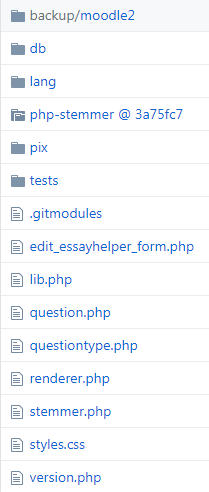
\includegraphics[scale=0.7]{images/architecture.png}
  \caption{Processus de racination Snowball pour la langue fran\c{c}aise.}
  \label{dev-architecture}
\end{figure}
\begin{description}
 \item[backup/moodle2]
 
 Fichier qui g\`ere la sauvegarde et la restauration des questions de ce type.
 Le sous-dossier moodle2 indique que cette fonctionnalit\'e existe seulement pour la version 2 de Moodle et les suivantes.
 
 \item[db]
 
 Contiens un fichier \og install.xml \fg{} qui d\'efinit la table de base de donn\'ees \`a cr\'eer pour ce module d'extension.
 
 \item[lang]
 
 Contient un sous-dossier par langue support\'ee sois \og fr \fg{} et \og en \fg{} dans ce projet.
 Chaque sous-dossier contient un fichier PHP qui d\'efini les cha\^ines de traductions.
 Ce dossier de traduction est valide pour les fonctionnalit\'es Moodle, pas pour la racination.
 
 \item[php-stemmer]
 
 Sous-module git pour ce projet uniquement.
 Pointe vers la librairie de racination utilis\'e et d\'ecrit au chapitre \ref{chap:phpstemmer}.
 
 \item[pix]
 
 Contiens l'ic\^one du type de question.
 Cette ic\^one est uniquement visible lorsque l'enseignant choisit le type de question pour une nouvelle question.
 
 \item[tests]
 
 Ce dossier contient tous les tests unitaires et d'acception du module d'extension.
 Pour plus de d\'etail, voir la section \ref{dev_test}.
 
 \item[edit\_essayhelper\_form.php]
 
 D\'efini le formulaire que l'enseignant remplis lorsqu'il cr\'e une question de ce type.
 Il faut uniquement d\'efinir les champs sp\'ecifiques au type de question actuel, Moodle ajoute ajoute automatiquement les champs de base comme le nom de la question et la valeur en point de la question dans le questionnaire.
 
 \item[question.php]
 
 G\`ere la r\'eponse \`a une question.
 D\'efini le comportement de question \`a utiliser, comment afficher la r\'eponse (appel renderer.php) et valide la pr\'esence d'une r\'eponse.
 
 \item[questiontype.php]
 
 G\`ere la cr\'eation, modification et suppression d'une question de ce type.
 
 \item[renderer.php]
 
 G\`ere l'affichage d'une question et des r\'eponses.
 Permets de contr\^oler la zone de texte pour une nouvelle r\'eponse ou pour la modifier.
 Permets aussi de changer l'affichage de la r\'eponse pour le correcteur.
 C'est dans ce fichier que nous allons surtout travailler.
 
 \item[stemmer.php]
 
 Fichier sp\'ecialement con\c{c}u pour ce module d'extension.
 C'est dans ce fichier que nous g\'erons le lien entre Moodle et \texttt{php-stemmer}.
 
 \item[styles.css]
 
 Fichier css pour notre module d'extension.
 
 \item[version.php]
 
 Fichier contenant 4 informations:
 \begin{itemize}
   \item \og component \fg{}
   
   Nom du module d'extension qui sera utilis\'e dans la base de donn\'ees Moodle.
   Dans ce projet il s'agit de \og qtype\_essayhelper \fg{}.
   
   \item \og version \fg{}
   
   Num\'ero de version du module d'extension dans le format \og aaaammjj00 \fg{} utilisant la date.
   Les deux derniers \og 0 \fg{} sont utilis\'es pour faire plus qu'une version par jour.
   Pour que Moodle prenne en compte les changements au fichier \og install.xml \fg{} (pour la base de donn\'ees), il faut changer le num\'ero de version.
   
   \item \og requires \fg{}
   
   Num\'ero de version Moodle n\'ecessaire au bon fonctionnement du module d'extension utilisant aussi le format \og aaaammjj00 \fg{}.
   Notre module d'extension utilise la m\^eme d\'ependance que \og qtype\_essay \fg{} soit \og 2015111600 \fg{} qui repr\'esente Moodle 3.0.
   
   \item \og maturity \fg{}
   
   La maturit\'e du module d'extension.
   Notre module d'extension se trouve encore en \textit{MATURITY\_ALPHA}.
 \end{itemize}
\end{description}
Dans tous les fichiers il y a eu un peu d'adaptation du code afin de passer de \og qtype\_essay \fg{} \`a \og qtype\_essayhelper \fg{}.
\section{Code Moodle de qtype\_essayhelper}
Le code du module d'extension est peu complexe.
Ce qui cause de la complexit\'e dans le projet r\'eside dans l'interaction entre le coeur de Moodle et ces classes.
La figure \ref{dev-class} illustre les diff\'erentes classes qui seront d\'etaill\'ees dans les prochaines pages.
\begin{figure}[h!]
  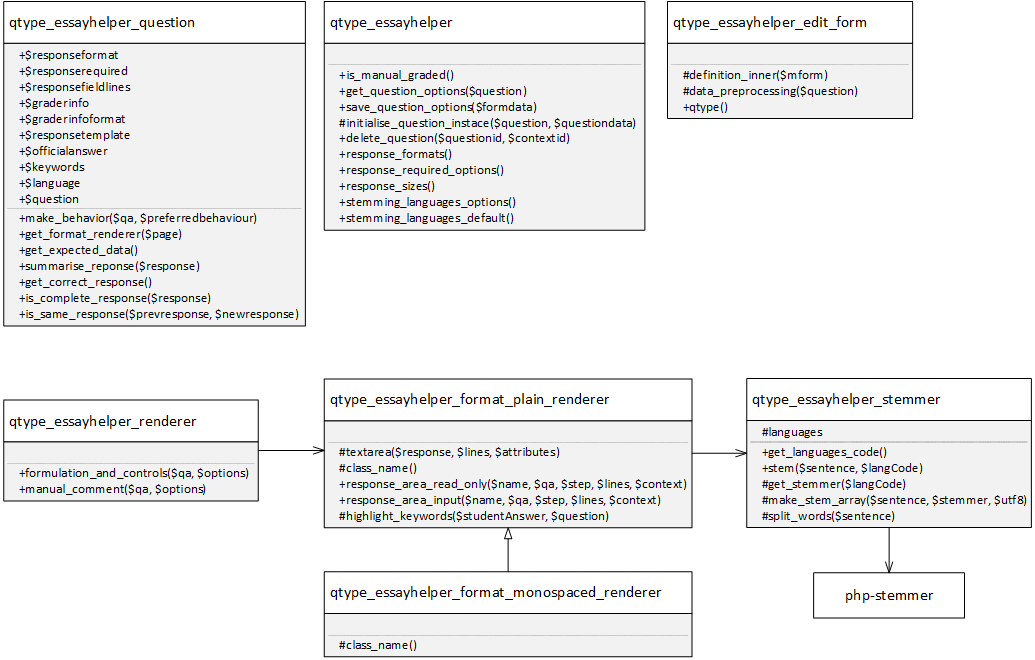
\includegraphics[scale=0.5]{images/class.png}
  \caption{Principales classes de \texttt{qtype\_essayhelper}.}
  \label{dev-class}
\end{figure}
\subsection*{Classe \texttt{qtype\_essayhelper\_edit\_form}}
Cette classe g\`ere le formulaire de cr\'eation et modification de question pour ce type de question.
Elle poss\`ede deux fonctions, la premi\`ere est \og definition\_inner \fg{} qui permet d'ajouter des champs au formulaire de base de cr\'eation de questions.
Le formulaire de base comporte quelques champs tels que le titre de la question, le texte de la question ainsi que le nombre de points que vaut cette question.
La gestion des champs de base se fait automatiquement par Moodle, il ne reste donc qu'\`a ajouter nos champs suppl\'ementaires pour notre type de question.
L'ajout de champs se fait avec un objet formulaire fourni par Moodle.
L'exemple de code \ref{code:formdefinition} illustre l'ajout des champs d'aide \`a la correction dans le formulaire de notre module d'extension.
La fonction principale de cet objet est addElement qui prend 4 param\`etres:
\begin{enumerate}
  \item Le type d'\'el\'ement;
  \item Le nom du champ doit \^etre le m\^eme que dans la base de donn\'ees;
  \item Le texte \`a afficher, la fonction \textit{get\_string} traduit la cha\^ine donn\'ee en premier param\`etre dans les fichiers de traductions du module d'extension donn\'e dans le deuxi\`eme param\`etre;
  \item Optionnellement, des options suppl\'ementaires.
\end{enumerate}
\begin{lstfloat}
\begin{lstlisting}[frame=l]
$qtype = question_bank::get_qtype('essayhelper');
$mform->addElement('header', 'essayhelper', get_string('essayhelperheader', 'qtype_essayhelper'));
$mform->setExpanded('essayhelper');
$mform->addElement('textarea', 'officialanswer', get_string('officialanswer', 'qtype_essayhelper'),
 array('rows' => 10, 'cols' => 100));
$mform->addElement('textarea', 'keywords', get_string('keywords', 'qtype_essayhelper'),
 array('rows' => 10, 'cols' => 60));
$mform->addHelpButton('keywords', 'keywords', 'qtype_essayhelper');
\end{lstlisting}
\caption{Extrait du code de la fonction definition\_inner de la classe qtype\_essayhelper\_edit\_form.}
\label{code:formdefinition}
\end{lstfloat}
La deuxi\`eme fonction de cette classe permet de sauvegarder les champs du formulaire.
Tous les champs non reconnus par Moodle doivent \^etre trait\'es manuellement dans cette fonction comme illustr\'ee \`a l'exemple de code \ref{code:formpreprocessing}.
\begin{lstfloat}
\begin{lstlisting}[frame=l]
$question->responsetemplate = $question->options->responsetemplate;
$question->officialanswer = $question->options->officialanswer;
$question->keywords = $question->options->keywords;
\end{lstlisting}
\caption{Extrait du code de la fonction data\_preprocessing de la classe qtype\_essayhelper\_edit\_form.}
\label{code:formpreprocessing}
\end{lstfloat}
\subsection*{Classe \texttt{qtype\_essayhelper\_question}}
Cette classe g\`ere la r\'eponse \`a une question, que ce soit pour une nouvelle r\'eponse, une modification de r\'eponse ou afficher la r\'eponse au correcteur.
Les fonctions d\'efinies dans cette classe sont:
\begin{description}
  \item[make\_behaviour] Retourne le comportement utilis\'e par le type de question. \texttt{manualgraded} dans ce cas.
  \item[get\_format\_renderer] Retourne la classe \texttt{qtype\_essayhelper\_renderer} qui s'occupera de l'affichage de la question.
  \item[get\_expected\_data] Retourne ce que la r\'eponse de l'\'etudiant doit contenir. Dans notre cas il y a seulement une r\'eponse textuelle.
  \item[summarise\_response] Retourne un r\'esum\'e de la r\'eponse de l'\'etudiant, dans notre cas il s'agit de la r\'eponse directement. Sera utilis\'e dans les modules de corrections afin de donner un aper\c{c}u de la r\'eponse de chaque \'etudiant.
  \item[get\_correct\_response] Devrait retourner la bonne r\'eponse \`a la question. Notre fonction retourne null afin d'indiquer \`a Moodle qu'il n'y a pas de bonne r\'eponse.
  \item[is\_complete\_response] V\'erifie si l'\'etudiant a r\'epondu \`a la question. Nous v\'erifions simplement s'il y a une r\'eponse non-vide.
  \item[is\_same\_response] D\'etermine si l'\'etudiant a modifi\'e sa r\'eponse.
\end{description}
\subsection*{Classe qtype\_essayhelper}
Cette classe g\`ere les options du type de question ainsi que les interactions \`a la base de donn\'ees.
Les fonctions d'interactions avec la base de donn\'ees:
\begin{description}
  \item[is\_manual\_graded] Retourne \texttt{vrai} dans notre cas pour indiquer que la question doit se corriger manuellement.
  \item[get\_question\_options] R\'ecup\`ere les options pour la question d\'efinie dans la base de donn\'ees. Nous retournons simplement le r\'esultat de la requ\^ete.
  \item[save\_question\_options] Ici il faut prendre les donn\'ees du formulaire et les ajout\'er dans la base de donn\'ees. G\`ere la cr\'eation et la modification de la question.
  \item[initialise\_question\_instance] Initialise l'instance de la question en ajoutant les options \`a l'objet repr\'esentant la question.
  \item[delete\_question] Supprime la question de la base de donn\'ees. Notre type de question n'utilise qu'une seule table, il s'agit donc d'une seule requ\^ete \texttt{DELETE}.
\end{description}
Les options du type de question sont des listes d\'eroulantes dans le formulaire de cr\'eation et modification de question.
Les fonctions qui d\'efinissent les options sont:
\begin{description}
  \item[response\_formats] Retourne les formats de r\'eponses possibles soit \og Texte pur \fg{} et \og Texte pur, police monospace \fg{} .
  \item[response\_required\_options] Retourne deux options soit \og Requiers la saisie d'un texte par le participant \fg{} et \og Saisie de texte optionnelle \fg{}.
  \item[response\_sizes] Donne le nombre de lignes par d\'efaut que contiendra le champ de r\'eponse. Nous donnons les options de 5 \`a 40 avec des intervalles de 5.
  \item[stemming\_languages\_options] R\'ecup\`ere toutes les langues disponibles pour la racination et les traduits dans la langue de l'utilisateur avec la fonction \texttt{PHP Locale::getDisplayName}.
  \item[stemming\_languages\_default] Trouve la langue de racination par d\'efaut en se basant sur la langue actuelle de l'utilisateur. Si la langue n'est pas reconnue, nous utilisons l'anglais.
\end{description}
\subsection*{Classe qtype\_essayhelper\_renderer}
Cette classe g\`ere l'affichage de la question aux \'etudiants lorsqu'ils r\'epondent ainsi que l'affiche de la r\'eponse de l'\'etudiant lors de la relecture de celui-ci ou lors de la correction.
Elle ne contient que deux fonctions:
\begin{description}
  \item[formulation\_and\_controls] G\`ere l'affichage du texte de la question, la zone de r\'eponse de l'\'etudiant est g\'er\'ee par la classe \texttt{ qtype\_essayhelper\_format\_plain\_renderer}.
  \item[manual\_comment] G\`ere l'affichage de la zone de commentaire de l'enseignant lors de la correction. Pour chaque r\'eponse l'enseignant peut laisser un commentaire.
\end{description}
\subsection*{qtype\_essayhelper\_format\_plain\_renderer}
Cette classe g\`ere la r\'eponse de l'\'etudiant.
\begin{description}
  \item[textarea] Fonction prot\'eg\'ee qui construit la zone de texte lorsqu'un \'etudiant r\'epond \`a la question.
  \item[class\_name] Fonction prot\'eg\'ee qui retourne le nom de la classe css \`a appliquer sur la balise \texttt{HTML} englobant la question et la r\'eponse.
  \item[response\_area\_read\_only] Fonction qui affiche le texte de la r\'eponse pour consultation seulement. Si c'est un enseignant ou un correcteur qui consulte la question dans le module de correction manuel on affiche la r\'eponse de l'enseignant \`a c\^ot\'e de la r\'eponse de l'\'etudiant et on met en \'evidence les mots clés
  \item[response\_area\_input] Affiche la zone de texte cr\'e\'e par la fonction \texttt{textarea} afin que l'\'etudiant puisse r\'epondre \`a la question.
  \item[highlight\_keywords] Met en \'evidence les mots-cl\'es trouv\'es dans le texte par la racination.
\end{description}
La classe \texttt{qtype\_essayhelper\_format\_monospaced\_renderer} hérite de la classe \texttt{qtype\_essayhelper\_format\_plain\_renderer} et red\'efini seulement la fonction \texttt{class\_name}.
Le CSS correspondant \`a la classe retourn\'ee est d\'efini dans le module d'extension \texttt{qtype\_essay}.
Un exemple de l'interaction de toutes ces classes avec Moodle est illustr\'e \`a la figure \ref{dev-diagramme}.
Cet exemple illustre l'ouverture d'un questionnaire par un \'etudiant.
\begin{landscape}
\begin{figure}[h!]
  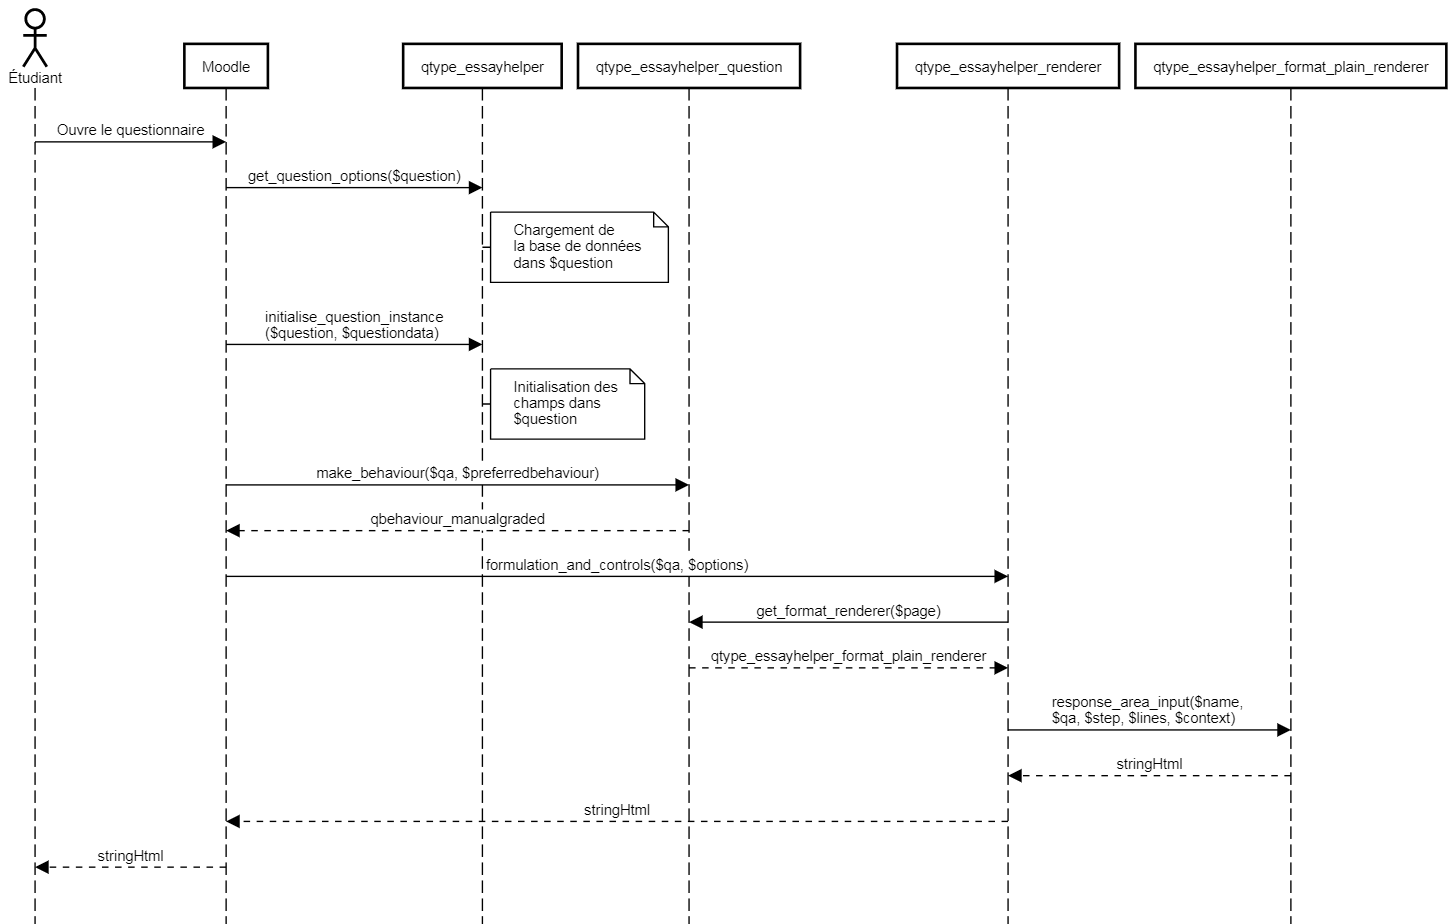
\includegraphics[scale=0.4]{images/diagramme-flux.png}
  \caption{Interaction entre Moodle et le module d'extension \texttt{qtype\_essayhelper}.}
  \label{dev-diagramme}
\end{figure}
\end{landscape}
\section{D\'etection des mots cl\'es}
Comme cit\'e dans le \autoref{chap:keywords}, nous utilisons la biblioth\`eque \texttt{php-stemmer} afin de trouver la racine de chaque mot.
Pour trouver la racine de tous les mots du texte, il faut d\'ebuter par les isoler.
Les caract\`eres non alphanum\'eriques sont remplac\'es par des espaces et le texte est d\'ecoup\'e par des caract\`eres d'espacement (espace, saut de ligne, tabulation, etc.) tel qu'illustr\'e dans l'extrait de code \ref{code:isoler}.
\begin{lstfloat}
\begin{lstlisting}[frame=l]
$words = preg_split('/(\s|\')/', preg_replace('/[^[:alnum:][:space:]]/u', ' ', $sentence));
\end{lstlisting}
\caption{Isoler les mots du texte.}
\label{code:isoler}
\end{lstfloat}
Ensuite, chaque mot est associ\'e avec sa racine trouv\'ee avec l'algorithme Snowball tel qu'illustr\'e dans l'extrait de code \ref{code:racinationsnowball}.
Chaque mot-cl\'e a, pr\'ealablement, aussi \'et\'e r\'eduit \`a sa racine avec l'algorithme Snowball.
\begin{lstfloat}
\begin{lstlisting}[frame=l]
foreach ($words as $word) {
 if ($word) {
  if (Wamania\Snowball\Utf8::check($word)) {
   $stem = $stemmer->stem($word);
   if (isset($stems[$stem])) {
    if (!in_array($word, $stems[$stem])) {
     $stems[$stem][] = $word;
    }
   } else {
    $stems[$stem] = array($word);
   }
  } else {
   $stems[] = $word;
  }
 }
}
\end{lstlisting}
\caption{Racination des mots avec Snowball.}
\label{code:racinationsnowball}
\end{lstfloat}
Finalement les mots-cl\'es trouv\'es dans le texte sont mis en \'evidence.
\begin{lstfloat}
\begin{lstlisting}[frame=l]
$usedKeywords = array_intersect(array_keys($stems), $keywords);
foreach ($usedKeywords as $keyword) {
 $words = $answerWords[$keyword];
 foreach ($words as $word) {
  $studentAnswer = str_replace($word, '<b><u>' . $word . '</u></b>', $studentAnswer);
 }
}
\end{lstlisting}
\caption{Mise en \'evidence des mots-cl\'es trouv\'es.}
\label{code:mots-cles}
\end{lstfloat}
\section{Tests} \label{dev_test}
Les tests du module d'extension \og qtype\_essay \fg{} ont \'et\'e conserv\'es et adapt\'es \`a ce nouveau module d'extension.
Le fonctionnement de base d'un module d'extension (cr\'eation de question, modification de question, r\'epondre \`a la question, etc.) a donc facilement \'et\'e test\'e.
Il ne restait plus qu'\`a tester les nouvelles fonctionnalit\'es de mots-cl\'es et d'affichage de la r\'eponse de l'enseignant.
\subsection{Tests d'acceptation} \label{dev_test_acceptation}
Les tests d'acceptation r\'ecup\'er\'es du module d'extension \textit{qtype\_essay} ont permis de trouver quelques probl\`emes  dans le nouveau module d'extension.
Par exemple, la fonctionnalit\'e \textit{Backup and restore} ne fonctionnait pas pour les questions avec le nouveau type de question \textit{qtype\_essayhelper}.
Le probl\`eme venait d'un dossier manquant dans le nouveau module d'extension.
Le dossier \textit{backup} dans le module d'extension \textit{qtype\_essayhelper} ne contiens pas des copies de sauvegardes du module d'extension, mais plusieurs versions de la fonctionnalit\'e \textit{Backup and restore}.
\subsection{Tests unitaires} \label{dev_test_unitaire}
La biblioth\`eque de racination \texttt{php-stemmer} est d\'ej\`a test\'e unitairement et valid\'e \`a l'aide d'un dictionnaire qui associe les mots \`a leurs racines.
Il ne restait donc qu'\`a tester l'int\'egration entre Moodle et la biblioth\`eque de racination.
\chapter{R\'esultats obtenus et limites de notre module de correction}
L'affichage de la r\'eponse de l'enseignant et de l'\'etudiant c\^ote \`a c\^ote, en plus des instructions au correcteur, devrait aider le correcteur dans sa t\^ache de correction.
De plus, la possibilit\'e de choisir la langue de racination permet aux enseignants d'utiliser l'aide \`a la correction dans la langue de leur choix.

\GT{Mentionner que pour l'instant, toutefois, aucun test/essai n'a
\'et\'e fait avec de vrais \'etudiants, que ce serait quelque chose
d'int\'eressant \`a faire, mais pas fait faute de temps, absence d'un
contexte o\`u faire de tels essais avec de vraies personnes, blah,
blah, etc.~;)}

Un probl\`eme a \'et\'e d\'etect\'e vers la fin du projet: la s\'eparation du texte en mots peut poser probl\`eme.
Plus pr\'ecis\'ement, on s\'epare chaque mot en utilisant les symboles non alphanum\'erique et les caract\`eres d'espacement.
Donc, le mot \og aujourd'hui \fg{} est consid\'er\'e comme deux mots, car l'apostrophe est un symbole non alphanum\'erique, alors que c'est en fait un seul mot.
Par contre, \og qu'autrui \fg{} est aussi consid\'er\'e comme deux mots, ce qui est correct dans ce cas.
De plus, comme le module d'extension supporte plusieurs langues, chaque langue comporte ses particularit\'es.
Par exemple, en anglais le mot \og \textit{wasn't} \fg{} est une compression des mots \og \textit{was} \fg{} et \og \textit{not} \fg{} ce qui ne sera pas bien g\'er\'e.
Toutefois, il nous semble que ce probl\`eme ne soit pas assez majeur pour cr\'eer des probl\`emes dans la majorit\'e des situations.
Ainsi, m\^eme si \og aujourd'hui \fg{} est consid\'er\'e comme deux mots, la mise en \'evidence se fera sur chacun de ces deux mots.
Et en anglais, les mots probl\'ematiques (comme \og \textit{wasn't} \fg{}) seront rarement utilis\'es comme mots-cl\'es.
Comme ce probl\`eme ne nous semble pas majeur et que la solution serait complexe \`a mettre en oeuvre --- par exemple, en rempla\c{c}ant la racination par la lemmatisation ou en faisant de l'analyse syntaxique ---, nous avons d\'ecidé de ne pas le traiter.

\`A la suite de l'analyse du probl\`eme pr\'ec\'edent, nous avons d\'ecouvert un deuxi\`eme probl\`eme.
Pour mettre en \'evidence les mots, on se base sur un dictionnaire qui associe le mot \`a la racine.
Si le mot-cl\'e est \og aimer \fg{} et le texte contient les mots \og aimera \fg{} et \og aimerait \fg{}, les deux mots seront mis en \'evidence.
Par contre, la partie du mot \og aimera \fg{} du mot \og aimerait \fg{} sera mise en \'evidence deux fois, car il contient l'autre mot qui doit \^etre mis en \'evidence.
La mise en \'evidence fait un simple remplacement de cha\^ine du mot par ce m\^eme mot entour\'e de balises \texttt{HTML} comme le d\'emontre l'exemple de code \ref{code:mots-cles}.
Une mise en \'evidence double ne sera pas diff\'erente visuellement d'une mise en \'evidence simple, car une balise de style \texttt{HTML} ou \texttt{CSS} dans une balise du m\^eme style ne fera pas de modification suppl\'ementaire.
En utilisant l'exemple pr\'ec\'edent, bien que \og aimerait \fg{} serait en partie mis en \'evidence deux fois, le mot ne sera soulign\'e qu'une seule fois.

Diverses am\'elioration pourraient aussi \^etre ajout\'ees au module d'extension.
Par exemple, la mise en \'evidence des mot-cl\'es est relativement simple; or, elle pourrait \^etre configurable via l'interface d'administration afin de changer le style de mise en \'evidence.
En ce moment la mise en \'evidence met simplement le mot en gras et soulign\'e.

La racination utilis\'ee est aussi limit\'ee~: le correcteur doit lire le contexte afin de confirmer si le mot-cl\'e est valide, probl\`eme qui pourrait \^etre \'elimin\'e avec un outil de lemmatisation.
De m\^eme, les mots-cl\'es originaux ne sont pas affich\'es au correcteur, ce qui pourrait \^etre un ajout int\'eressant.

Finalement, dans la planification initiale du projet, il \'etait pr\'evu de pouvoir comparer les textes des \'etudiants entre eux --- au lieu de seulement les comparer au texte de l'enseignant.
Dans un premier temps, nous voulions simplement afficher les r\'eponses des autres \'etudiants \`a la place de la r\'eponse de l'enseignant afin de comparer les r\'eponses semblables.
Par contre, cette id\'ee demandait une analyse syntaxique afin de trouver les r\'eponses semblables, ce qui sortait du cadre du projet.
Cet ajout pourrait \^etre un projet int\'eressant pour un futur \'etudiant.

Ces limitations font en sorte qu'il ne nous semble pas encore appropri\'e de soumettre
notre module au r\'epertoire officiel des modules d'extension Moodle.
Toutefois, apr\`es am\'eliorations, il pourrait devenir un ajout int\'eressant pour les enseignants et correcteurs du monde entier.

Signalons que
le code source de notre module est quand m\^eme disponible sur GitHub comme le stipule les r\`egles de d\'eveloppement Moodle, \`a l'adresse \url{https://github.com/Padreik/moodle-qtype_essayhelper}.


\begin{conclusion}
Dans ce projet, initialement d'apparence plut\^ot simple, plusieurs points ont \'et\'e sous-estim\'es.
Premi\`erement, la cr\'eation de modules d'extension Moodle diff\`ere de mon exp\'erience en mati\`ere de module d'extension \texttt{PHP} avec Wordpress et Typo3.
Moodle est un syst\`eme complexe, ce qui se refl\`ete dans son code et ses modules d'extension.
L'interaction entre le module d'extension et Moodle n'est pas toujours claire et aurait d\^u \^etre analys\'ee plus en d\'etail au d\'ebut du d\'eveloppement.
Deuxi\`emement, l'organisation et la planification du temps a \'et\'e une source de difficult\'e.
Contrairement \`a un cours o\`u le projet peut/doit \^etre r\'ealis\'e en quelques jours --- au pire quelques semaines --- , ce projet s'est \'etendu sur plusieurs mois.
L'\'equilibre entre travail r\'emun\'er\'e,  vie priv\'ee et r\'ealisation de ce projet acad\'emiqe a \'et\'e une source de difficult\'e, parfois au d\'epend du projet.
Finalement, l'\'ecriture de ce rapport a n\'ecessit\'e plus de travail que pr\'evu.
L'\'ecriture n'\'etant pas ma force et ayant rarement \'ecrit des textes de plus de 5--10 pages, l'\'ecriture de ce rapport a \'et\'e un important d\'efi.

Ces difficult\'es que j'ai rencontr\'ees et, en partie, surmont\'ees vont, je l'esp\`ere, m'aider dans ma vie professionnelle:
\begin{itemize}
  \item \`A mieux analyser les syst\`emes inconnus avant de me lancer dans un projet;
  \item \`A mieux g\'erer mon horaire de fa\c{c}on plus efficace;
  \item \`A m'aider dans l'\'ecriture de rapports et de notes de cours.
\end{itemize}
J'esp\`ere aussi qu'en enseignant les cours de Web au c\'egep et en utilisant r\'eguli\`erement Moodle, les apprentissages faits dans le cadre de ce projet vont m'aider dans ma carri\`ere d'enseignant.
\end{conclusion}

% Utilisez l'environnement  conclusion pour rédiger votre conclusion

%%%%%%%%%%%%%%%%%%%%
% Page liminaires
%%%%%%%%%%%%%%%%%%%%

\appendix
\chapter{Test d'acceptation existant dans Moodle}
\label{annexe_behat_exist}

\begin{lstlisting}[language=behat,frame=l]
@qtype @qtype_essay
Feature: Test creating an Essay question
  As a teacher
  In order to test my students
  I need to be able to create an Essay question

  Background:
    Given the following "users" exist:
      | username | firstname | lastname | email               |
      | teacher1 | T1        | Teacher1 | teacher1@moodle.com |
    And the following "courses" exist:
      | fullname | shortname | category |
      | Course 1 | C1        | 0        |
    And the following "course enrolments" exist:
      | user     | course | role           |
      | teacher1 | C1     | editingteacher |
    And I log in as "teacher1"
    And I am on "Course 1" course homepage
    And I navigate to "Question bank" node in "Course administration"

  Scenario: Create an Essay question with Response format set to 'HTML editor'
    When I add a "Essay" question filling the form with:
      | Question name            | essay-001                      |
      | Question text            | Write an essay with 500 words. |
      | General feedback         | This is general feedback       |
      | Response format          | HTML editor                    |
    Then I should see "essay-001"

  Scenario: Create an Essay question with Response format set to 'HTML editor with the file picker'
    When I add a "Essay" question filling the form with:
      | Question name            | essay-002                      |
      | Question text            | Write an essay with 500 words. |
      | General feedback         | This is general feedback       |
      | Response format          | HTML editor                    |
    Then I should see "essay-002"
\end{lstlisting}

\chapter{Test d'acceptation de \texttt{qtype\_essayhelper}}
\label{annexe_behat_new}

\begin{lstlisting}[language=behat,frame=l,style=default]
@qtype @qtype_essayhelper
Feature: Validate Essay with correction helper special features
  As a teacher
  In order to be helped correcting essays
  I need to see teacher answer and keywords while correcting while students don't

  Background:
    Given the following "users" exist:
      | username | firstname | lastname | email               |
      | teacher1 | T1        | Teacher1 | teacher1@moodle.com |
      | student1 | S1        | Student1 | student1@moodle.com |
    And the following "courses" exist:
      | fullname | shortname | category |
      | Course 1 | C1        | 0        |
    And the following "course enrolments" exist:
      | user     | course | role           |
      | teacher1 | C1     | editingteacher |
      | student1 | C1     | student        |
    And the following "question categories" exist:
      | contextlevel | reference | name           |
      | Course       | C1        | Test questions |
    And the following "questions" exist:
      | questioncategory | qtype       | name      | template |
      | Test questions   | essayhelper | essay-001 | plain    |
    And the following "activities" exist:
      | activity   | name   | course | idnumber |
      | quiz       | Quiz 1 | C1     | quiz1    |
    And quiz "Quiz 1" contains the following questions:
      | question   | page |
      | essay-001  | 1    |

  @javascript
  Scenario: A student submit an Essay with correction helper answer and don't see the correction helper.
    When I log in as "student1"
    And I am on "Course 1" course homepage
    And I follow "Quiz 1"
    And I press "Attempt quiz now"
    Then I should not see "Teacher answer" on quiz page "1"
    And I follow "Finish attempt ..."
    And I press "Submit all and finish"
    And I click on "Submit all and finish" "button" in the "Confirmation" "dialogue"
    Then I should see "Finished"
    Then I should not see "Teacher answer" on quiz page "1"

  @javascript
  Scenario: A teacher should see the correction helper while manually grading.
    # Create answer
    Given I log in as "student1"
    And I am on "Course 1" course homepage
    And I follow "Quiz 1"
    And I press "Attempt quiz now"
    And I set the field with xpath "//textarea[contains(@class, 'qtype_essayhelper_response')]" to "I think it's a frog"
    And I follow "Finish attempt ..."
    And I press "Submit all and finish"
    And I click on "Submit all and finish" "button" in the "Confirmation" "dialogue"
    And I log out

    # Go to manuel correction module
    And I log in as "teacher1"
    And I am on "Course 1" course homepage
    And I follow "Quiz 1"
    And I navigate to "Results > Manual grading" in current page administration
    And I should see "Manual grading"
    And I click on "grade all" "link" in the "essay-001" "table_row"
    Then I should see "Teacher answer"

    # Test Keyword
    Then "//b/u[contains(text(), 'frog')]" "xpath_element" should exist
\end{lstlisting}

\chapter{Exemple de test unitaire de \texttt{qtype\_essayhelper}}
\label{annexe_unittest}

\begin{lstlisting}[language=php,frame=l,style=default]
class qtype_essayhelper_stemmer_test extends basic_testcase {
    public function test_get_stemmer_all_languages_exists() {
        $stemmer = new qtype_essayhelper_stemmer();

        // Set get_stemmer function accessible
        $get_stemmer = $this->get_protected_function($stemmer, "get_stemmer");

        // Get all available languages
        $languages = PHPUnit\Framework\Assert::readAttribute($stemmer, "languages");

        // Test all languages
        foreach ($languages as $langCode => $lang) {
            $langStemmer = $get_stemmer->invokeArgs($stemmer, array($langCode));
            $this->assertEquals((new \ReflectionClass($langStemmer))->getShortName(), $lang);
        }
    }

    public function test_get_stemmer_language_non_existing() {
        $stemmer = new qtype_essayhelper_stemmer();

        // Set get_stemmer function accessible
        $get_stemmer = $this->get_protected_function($stemmer, "get_stemmer");

        // Test non existing language
        $langStemmer = $get_stemmer->invokeArgs($stemmer, array("zzz"));
        $this->assertEquals((new \ReflectionClass($langStemmer))->getShortName(), "English");
    }

    public function test_split_words_no_words() {
        $stemmer = new qtype_essayhelper_stemmer();
        $split_words = $this->get_protected_function($stemmer, "split_words");

        $this->assertEquals($split_words->invokeArgs($stemmer, array("")), array());
        $this->assertEquals($split_words->invokeArgs($stemmer, array("-\n    ' %")), array());
    }

    public function test_split_words_couple_words() {
        $stemmer = new qtype_essayhelper_stemmer();
        $split_words = $this->get_protected_function($stemmer, "split_words");

        $this->assertEquals($split_words->invokeArgs($stemmer, array("I love potatoes")), array("I", "love", "potatoes"));
        $this->assertEquals($split_words->invokeArgs($stemmer, array("I+love+potatoes")), array("I", "love", "potatoes"));
        $this->assertEquals($split_words->invokeArgs($stemmer, array("I-love\npotatoes")), array("I", "love", "potatoes"));
    }

    public function test_split_words_a_lot_of_words() {
        $stemmer = new qtype_essayhelper_stemmer();
        $split_words = $this->get_protected_function($stemmer, "split_words");

        $this->assertEquals($split_words->invokeArgs($stemmer,
            array("strap complex obtainable marked credit women wary educate nation wonder
              lours singulier musicien bannière lotus actrice premier polluer dans vie")),
            array("strap", "complex", "obtainable", "marked", "credit", "women", "wary", "educate",
                "nation", "wonder", "lours", "singulier", "musicien", "bannière", "lotus", "actrice",
                "premier", "polluer", "dans", "vie"));
    }

    public function test_make_stem_array() {
        $stemmer = new qtype_essayhelper_stemmer();
        $make_stem_array = $this->get_protected_function($stemmer, "make_stem_array");

        // The stem for all words will be "test"
        $snowball_stemmer = $this->createMock('\\Wamania\\Snowball\\Stemmer', array('stem'));
        $snowball_stemmer->method('stem')->willReturn('test');

        $snowball_utf8 = new qtype_essayhelper_stemmer_utf8_mock();

        $make_stem_array = $this->get_protected_function($stemmer, 'make_stem_array');

        $stemmed_array = $make_stem_array->invokeArgs($stemmer, array("test asdf", $snowball_stemmer, $snowball_utf8));
        $expected_stemmed_array = array("test" => array("test", "asdf"));

        $this->assertEquals($stemmed_array, $expected_stemmed_array);
    }

    protected function get_protected_function($stemmer, $protectedFunctionName) {
        $reflection = new ReflectionClass($stemmer);
        $protectedFunction = $reflection->getMethod($protectedFunctionName);
        $protectedFunction->setAccessible(true);
        return $protectedFunction;
    }
}

class qtype_essayhelper_stemmer_utf8_mock extends Wamania\Snowball\Utf8 {
    public static function check($str) {
        return true;
    }
}
\end{lstlisting}
\nocite{*}
\bibliographystyle{apalike-uqam}
\bibliography{bibliographie}
\end{document}
